% Created 2020-09-23 Wed 10:18
\documentclass[9pt, b5paper]{article}
\usepackage[UTF8]{ctex}
\usepackage{fontspec}
\usepackage{graphicx}
\usepackage{xcolor}
\usepackage{multirow}
\usepackage{multicol}
\usepackage{float}
\usepackage{textcomp}
\usepackage{geometry}
\geometry{left=1.2cm,right=1.2cm,top=1.5cm,bottom=1.2cm}
\usepackage{algorithm}
\usepackage{algorithmic}
\usepackage{latexsym}
\usepackage{natbib}
\usepackage{listings}
\usepackage{minted}
\usepackage[xetex,colorlinks=true,CJKbookmarks=true,linkcolor=blue,urlcolor=blue,menucolor=blue]{hyperref}
\author{Deepwaterooo Wang}
\date{\today}
\title{打着爱国的旗号利用人的、与被利用的 \&\& 打着爱国的旗号逼良为娼的、与顽强反抗的}
\hypersetup{
  pdfkeywords={},
  pdfsubject={},
  pdfcreator={Emacs 27.1 (Org mode 8.2.7c)}}
\begin{document}

\maketitle
\tableofcontents


\section{关键人物及相互关系}
\label{sec-1}
\subsection{KC Wang(王孔启) @WSU}
\label{sec-1-1}

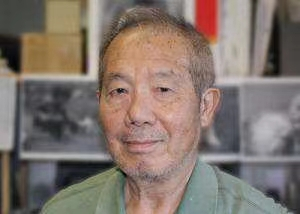
\includegraphics[width=.9\linewidth]{./pic/KCWang.jpg}
\begin{itemize}
\item \url{https://school.eecs.wsu.edu/faculty/profile/?nid=kwang}
\item 王孔启:1936年9月24日出生,属鼠天秤座人,当时阶级成分:地主。在五十年代左右斗地主的阶级斗争中,随其地主父亲辗转移居台湾,后留学美国并于美国定居,生下三子。次子Eric Wang。
\end{itemize}
\subsection{Sherry Wang (王夏华) @Samsung}
\label{sec-1-2}

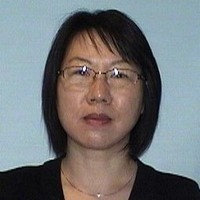
\includegraphics[width=.9\linewidth]{./pic/Sherry Wang.jpg}
\begin{itemize}
\item \url{https://www.linkedin.com/in/xhswang/}
\item Sherry Wang (王夏华):1963年生属兔魔羯座,国内读高中但第一年没有考上大学;复读一年后也只考了个大专;毕业后在襄阳电大技校教书,结果被裁员,其父王孔庚跑动所有的关系,才又保住其在襄阳电大一个教员的位置。98年Cindy Wang生产第一个小孩时随其母来美,之后没有回中国,申请了加拿大绿卡。在KC Wang的帮助下入WSU读计算机专业硕士。2000年毕业,学生身份到期回加拿大干了七年体力工,于2007年44岁时再次回美,并在Cindy Wang的帮助下开启工作人生,先后曾在Cisco和另一家公司上过班,第三家便被敏感地回入到了以做广告创意闻名于世的Samsung,2013年时在三星工作。至此被三星公司包养送终、2014、2015年特意为其加持出差西雅图并为其办绿卡。并在其的refer下将其自己的子Ben He/Huo从加拿大空降至苹果公司工作。
\end{itemize}
\subsection{Eric Wang @WSU}
\label{sec-1-3}

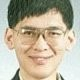
\includegraphics[width=.9\linewidth]{./pic/Eric Wang.jpg}
\begin{itemize}
\item Eric Wang:1966年6月17日出生,属马双子座人。大学研究生期间与无数女生有染,数次被停学,终于一韩国导师带至韩国在实验室做助理研究员,至2009年秋季重回WSU读博士。
\end{itemize}
\subsection{Ben Huo(He) (贺、霍笨笨?) @Apple}
\label{sec-1-4}
\begin{itemize}
\item 王夏华的独子
\end{itemize}
\subsection{Cindy Wang王秋勤 @Brocade}
\label{sec-1-5}
\begin{itemize}
\item \url{https://www.linkedin.com/in/cindy-wang-0420b66/}
\item 王孔启的侄女,王夏华的同父同母妹妹
\item Cindy Wang王秋勤:八十年代读高一高二时被其母请求王孔启将其带至美国读高中、大学和硕士,后因加入89年六四动乱留学生游行获批美国绿卡。
\end{itemize}
\subsection{王孔庚(中国大陆)}
\label{sec-1-6}
\begin{itemize}
\item 王孔启的亲哥哥,王夏华的父亲
\end{itemize}


\section{关键从物: 王孔启 KC Wang}
\label{sec-2}
\begin{itemize}
\item 冷酷无情,为谋家庭利益,为了其儿子Eric Wang 能够在WSU保住一个教职职位(最终其得到了)、为了其侄女王夏华Sherry Wang能够舒服一点儿地在美国生存下来(44岁才开记的人生第一份工作、后被三星公司包养),为了其侄孙何/贺笨笨的未来(也被从加拿大空降至苹果公司工作),不惜发动阶级战争,挥舞着爱国的大旗,对别人的人生实施灾难性的打击。
\begin{itemize}
\item 学习工作职业发展上:97年夏天劝我读农林院校;2001年我大三,很希望能够出国留学,写电子邮件给他,他没有回我的邮件;待别人2006年来美在读博时,却去劝阻别人读博,经济担保别人去读硕;别人是学生,本该好好努力学习时,却被他2008年夏天带至加州Cindy Wang家,说是带别人去加州大城市打工,实则向王夏华及其父母传达要她好好利用我以便王夏华能够轻松地在美国生存下来之意。其当着所有一圈并人拍着胸脯向王夏华及其父母保证,他能屐他的势力保证他家侄女王夏华能够轻轻松松在美国生存下来。却把正利用的别人使劲往偏路上引和逼。
\item 感情上:2010年更是,别人对他家老二根本没什么意思,他却还要故意说美国人可不在意你们是不是近亲,再说你们近亲也是超过三代,美国法律又没有不允许近亲结婚。呵呵,好不一“没有不允许”,却一再把别人往歧途上推,在别人根本不曾喜欢、不喜欢他家老二时,狠狠地把别人往火炕里一把狠推。从2010年到2015年,白白浪费了别人数年的青春。
\end{itemize}
\end{itemize}
\subsection{他侄女的所有的一切都是对的,而我所有的一切都是错的}
\label{sec-2-1}
\subsection{为家族利益、设计祸害别人的人生}
\label{sec-2-2}
\begin{itemize}
\item 至此,王孔启KC Wang刻意设计情节,如劝阻别人读博,经济担保别人去读硕士,如安排他的二儿子Eric Wang 2009年秋天回WSU读博,还发动一场所谓的恋爱,也都不过是他为了他亲侄女王夏华在美国的生存而采取的政治投机手段而已。呵呵,曾经的一场恋爱,现在只要一回想都会犯恶心。

\item 试问有谁见曾过这么变态的恋爱?既是他王孔启KC Wang要求别人多回去,又要嫌别人骚扰;既是他们发起恋爱的攻势,又是他残忍、冷酷无情地以911来严酷镇压;既是他虚伪地标榜着让别人去探索、寻求别人的人生,同样还是他已经一次又一次地对别人的人生一次次祸害加害以达到他政治投机的目的。

\item 地主是什么,地主是自私自利、黑良心、没有道德,赤裸裸地剥削别人的剩余价值。而他王孔启作为五十年代大环境头地主时代下当地大地主的儿子,无疑他如此残忍地操纵、加害别人人生的作法就是他作为地主的儿子的天然生物本能。呵呵,摇什么爱国的大旗,一个十足的小丑而已。

\item 事态发展到这一步,无疑,他王孔启KC Wang作为地主儿子的手段足够残忍,他的套路够深,以至于他的政治投机能够短暂得逞。可事态会如何发展呢?生于天秤座的王孔启自然是懂得平衡的。一开始就是设计利用别人,一开始就已经采取了诛心行动了。到时也不过别人不愿意,当父母的又能怎样?他们家族便 -- 万事大吉(他的儿子得到教职工作了,他的亲侄女王夏华一家已然已经在美国轻松生存下来了。不仅如此,美国政府还负责买单,尽最大努力替王夏华一家保密消息操守操行,她2009年2010年与公司男同事不清不楚的所有的银荡都可以被掩饰洗刷的如白雪公主一般清白,她在以广告创意闻名于世的三星公司的工作王夏华得到的也就像是王夏华凭借自已非凡的努力自己挣得的一样!呵呵)。而这一场地主儿子龟孙子王孔启KC Wang 对别人人生的祸害加害,便换来了他所谓忠心耿耿的爱国,换来了他家亲侄女王夏华一家人在美国的轻松生存。而他,一个没有道德的人,对于他所祸害、加害、伤害到的别人的人生,没有哪怕一丝的愧疚,付不起半点儿的责任。

\item 而这,便是当下美国最近十年所发生的一场赤裸裸的政治投机、阶级谋杀。只因为我是国际留学生,只因为我被他王孔启KC Wang利用,曾经与他的儿子谈过一场被他们父子精心设计的所谓恋爱,我的人生便该遭此天劫,那么谁来为道德摇旗,谁来为人生的正义买单?
\end{itemize}
燕:
\subsection{政治投机}
\label{sec-2-3}
\begin{itemize}
\item KC Wang打着爱国的旗号,行政治投机之事。
\item 2008年夏天在王秋勤处,向王夏华及其父母传达他把可以利用的人已经交到他们手上,要王夏华好好利用我以得以在美国轻松生存下来之意。其所在的一周,王夏华每晚故意拖到晚上11点多才回家,其周四的晚上就等到11点多直接等到王夏华回来向其转达不需要她王夏华工作太辛苦,他王孔启保证发动所有他能够发动的势力,保证王夏华能够在美国轻松生存下来之意。
\item KC Wang打着爱国的旗号,可以猜测应该是说着绝不为自己谋私利的话,实则从我2006年来美,他的办公室从来都挂着王夏华Sherry Wang作为WSU学生时的巨幅大头照。说王夏华Sherry Wang 2007年44岁才得到职业生涯里第一份工作、期间两三份工作都是老板上司的提携、2015年便被三星公司故意加持出差、包养养老送终给办绿卡、这样的职业发展不是他王孔启KC Wang政治投机的结果,你信吗?
\item 细看台湾这一族人作为斗地主大环境下外逃地主及其后代的集中营,其投机成分、现象和比例有多严重?我曾遇到Palo Alto一对双胞胎的母亲作为来自台湾的加拿大后裔,为争夺婆家所在palo alto两套房产对长相像父亲的幼子无所不用其极地虐待的恶劣行径,加上KC Wang的政治投机,现在对台湾这一族及后人已是深恶痛绝。
\item 在KC Wang 发动的这场政治投机里,所有的好处他KC Wang家(Eric Wang在WSU里的教职职位)、Sherry Wang的职业发展以及被三星公司包养养老送终的既定事实、Ben Huo/He被从加拿大空降至苹果公司工作的既定事实,所有的好处他们家占尽了,而所有的坏处、不能得到工作、不允许别人工作却要被利用的人独自承担。美国的政治居然如此,阶级斗争居然如此,对国际留学生的打压绝无公平可言,政治管理者居然也都这么无能,明摆着是KC Wang为了家族私利的一场政治投机,却还要一而再、再而三地为王夏华、王秋勤家(两个孩子的大学研究生前途)投放政治利益。
\end{itemize}

燕:
\subsection{他侄女王夏华的所有的一切都是对的,而被利用的人所做的一切都是错的}
\label{sec-2-4}
\begin{itemize}
\item 2010年我在加州时王夏华带我去银行办可以返\$50 \$100的信用卡,因为我同时办借记卡,而当时初入职场的的我还没有什么收入,银行开户时问她借了\$1000多块钱。后来王夏华几次三番地逼别人还。别人没有经济上的安全感,稍微晚一点儿就不行。后来我还了。但这事在2010年回WSU时的王孔启KC Wang的眼里,就全成了我的错,饭桌上一直只批评我。所有的错都是我的错,而他家王夏华所有的做法都是对的
\item 他们家既有王孔启心机深重的、循序渐近地一个人物一个人物地出场(王孔启,Eric Wang与其母同时出现,再则Eric之弟粉墨登场),既有KC Wang不分青红皂白只批评自己(他家王夏华怎么做都是对的),又有离家出走、出逃多年不归的三儿媳妇的既定事实
\end{itemize}

利用人的与被利用的

\section{关键从物: 王孔启}
\label{sec-3}
\begin{itemize}
\item 冷酷无情,为谋家庭利益,为了其儿子Eric Wang 能够在WSU保住一个教职职位(最终其得到了)、为了其侄女王夏华Sherry Wang能在舒服一点儿地生存下来(44岁被三星公司包养了),为了其侄孙何(贺)笨笨的未来(也被从加拿大空降至苹果公司工作),不惜发动阶级战争,挥舞着爱国的大旗,对别人的人生实施灾难性的打击。
\begin{itemize}
\item 学习工作职业发展上:97年夏天劝我读农林院校;2001年我大三,很希望能够出国留学,写电子邮件给他,他没有回我的邮件;待别人2006年来美在读博时,却去劝阻别人读博,经济担保别人去读硕;别人是学生,本该好好努力学习时,却被他2008年夏天带至加州Cindy Wang家,说是带别人去加州大城市打工,实则向王夏华及其父母传达要她好好利用我以便王夏华能够轻松地在美国生存下来之意。其当着所有一圈并人拍着胸脯向王夏华及其父母保证,他能屐他的势力保证他家侄女王夏华能够轻轻松松在美国生存下来。把别人往偏路上引。
\item 感情上:2010年更是,别人对他家老二根本没什么意思,他却还要故意说美国人可不在意你们是不是近亲,再说你们近亲也超过三代,美国法律又没有不允许近亲结婚。呵呵,好不一“没有不允许”,却一再把别人往歧途上推,在别人根本不曾喜欢、不喜欢他家老二时,狠狠地把别人往火炕里一把狠推。从2010年到2015年,白白浪费了别人数年的青春。
\end{itemize}
\end{itemize}

\section{关键人物:王夏华}
\label{sec-4}
\begin{itemize}
\item 97年之前我不清楚,但97年至2000零几年的夏天,王孔启都在他曾经的家乡湖北省襄阳市宜城市朱市镇镇上王孔庚的家过夏天。关于王夏华如果来美在美国如何才能够生存下来,他们两家人一族人应该是深思熟虑,就其可能性讨论过无数次了。
\begin{itemize}
\item 2005年秋冬我申请美国的学校,数年不曾谋面的王夏华父母赴美之前却还能在北京饭店里请我吃饭,并将我美国五所学校的申请材料随其旅行箱亲自带至美国加州再分寄出去。
\item 2005年我所申请的美国五所学校,都是Cindy Wang通过电子邮件推荐的,包括WSU和UI
\item 2006年秋我赴美读书,感恩节打电话至加州王夏华母亲处,其母电话里反复重申:他们早就已经告诉过王孔启我在旁边学校读书,怎么他还没有来找你?
\item 2008年夏天KC Wang王孔启带我至加州王秋勤Cindy Wang处大城市打工。说的是要带我去大城市打工,实则王孔启是传达要求王夏华好好利用我以使其在美国能够轻松生存下来之意。王孔启当着一众亲人的面,当着五夏华及其父母的面,拍着胸脯说他保证他能够发动他所能够发动的势力,以使他家五夏华能够在美国轻松地生存下来
\item 2008年夏天,王夏华父母当着KC Wang王孔启的面,告诉我,他们(王夏华的父亲和母校)绝对不会允许我放弃读博而转读硕士。经济担保我读硕士是王孔启KC Wang在祸害别人的人生。王孔启没有任何可反驳、反对的。
\item 2015年我回加州时,王秋勤还为王孔启说话,说其就是那么个拎不清。但她的说辞此地无银三百两。
\end{itemize}
\end{itemize}


\section{关键从物: 王孔启}
\label{sec-5}
\begin{itemize}
\item 冷酷无情,为谋家庭利益,为了其儿子Eric Wang 能够在WSU保住一个教职职位(最终其得到了)、为了其侄女王夏华Sherry Wang能在舒服一点儿地生存下来(44岁被三星公司包养了),为了其侄孙何(贺)笨笨的未来(也被从加拿大空降至苹果公司工作),不惜发动阶级战争,挥舞着爱国的大旗,对别人的人生实施灾难性的打击。
\begin{itemize}
\item 学习工作职业发展上:97年夏天劝我读农林院校;2001年我大三,很希望能够出国留学,写电子邮件给他,他没有回我的邮件;待别人2006年来美在读博时,却去劝阻别人读博,经济担保别人去读硕;别人是学生,本该好好努力学习时,却被他2008年夏天带至加州Cindy Wang家,说是带别人去加州大城市打工,实则向王夏华及其父母传达要她好好利用我以便王夏华能够轻松地在美国生存下来之意。其当着所有一圈并人拍着胸脯向王夏华及其父母保证,他能屐他的势力保证他家侄女王夏华能够轻轻松松在美国生存下来。把别人往偏路上引。
\item 感情上:2010年更是,别人对他家老二根本没什么意思,他却还要故意说美国人可不在意你们是不是近亲,再说你们近亲也超过三代,美国法律又没有不允许近亲结婚。呵呵,好不一“没有不允许”,却一再把别人往歧途上推,在别人根本不曾喜欢、不喜欢他家老二时,狠狠地把别人往火炕里一把狠推。从2010年到2015年,白白浪费了别人数年的青春。
\end{itemize}
\end{itemize}


KCW@WSU:其特点如下: 
政治投机:把我当作了握在他手中的政治资源加以利用,为了其儿子王心选Eric Wang@WSU在学校一个教职职位、为其侄女王夏华Sherry Wang@Samsung及其侄孙贺、霍笨笨Ben Huo@Apple在美国的生存发展谋取福利,不惜一再加害别人的人生。其中包括恶意、故意阻拦别人读博士、以经济担保促使别人读硕士以进一步阻拦别人在美国的生存发展及为其亲人谋福利。
手段奸诈、没有诚意:
其为达到政治投机的目的所采取的手段是以其儿子为诱饵、打着爱国的旗号、披着爱情的外衣,掩耳盗铃,自欺欺人,对我这样一个作为其远亲的国际留学生恶意施加了赤裸裸的人生误导和伤害。
09年春天我因为情感问题拿着前前男友的生肖星夜去找他时,他话里有话地说得很清楚,相处的时候就随他的愿望和他在一起,现在还不定心,不管等他五年十年,都等他最终定心,到时他自然愿意和你在一起。到时,只要两个人能走到一起,不管到时还能不能有孩子,能有孩子当然再好不过,实在要不到两个人能安安稳稳地过完这辈子也挺好的。对于当时他的谆谆教诲,他是在说我与当时跟我年龄一般大的前前男友吗,他这个人无处不在、借助一切机会造势说的全是关于他自己的那个不成气的宝贝二儿子呀
2009年及这之前的几个夏天他都去韩国过暑假,为的便是说服其次子EW能够2009年秋天回美读博,这样其儿子会与我有在相邻城市一个学期的overlap方便他们操作探听操控。其间他假惺惺邀请我到他们家作客过两次,诱导我与他家儿子谈恋爱,假惺惺示意他们多希望我能够成为他们的儿媳妇,其求我毕业后还应该经常开车回来这个家。但到别人真开车回来时,其奸诈嘴脸毕现,强扣给别人一顶“不择手段”的帽子,实则KCW他自己才是这样一个不择手段、自导自演操控着这一切的进展(阻别人读博、故意把别人带偏等等),左右缝源、左右摇摆,不管他采取如何强硬的强盗手段,只要他从语言上、从他所挖的坑里,从他自己人为制造的障碍里能够把我逼到无路可走、因为我所谓的“不择手段”品格低劣便有苦有冤无处述,他的所谓的正义、他一直打着的所谓的爱国旗号便能帮他达到他所想要达到的一切目的,并通过他先发制人地挖好的坑、已经强扣到了别人头上的帽子、已然造就好了的势来保护他及其儿子不至于陷于任何于他们不利的困境中。
左右摇摆不定、打太极、摆脱责任与担当:
在继我2010年回学校办理了OPT延期后2011年2月再回去满足了他之前语言上明确对我要求过的要我工作以后多开车回家去看看的期望后,他便掌握了主动,他的立场也便开始一直在变。他不再如之前真诚,而是手段狠辣,直接像是变了一个人,心狠手辣地暴烈播打911,还要以没有用一杆枪把我崩了就是他对我这个远亲的最大仁慈来继续诱惑挽留别人的心,打着所谓大义、深情的晃子,实则是一再利用别人的痴情,这与红楼梦中狠毒王熙凤毒设相思局有什么区别,实在是造孽。
及至2011年我的OPT实习第二年即将结束,他及其儿子以往的和实际正在使用的极端手段就变成了推脱他一切责任的手段和护身符,把他及其儿子反复利用、蹂涅别人情感的道德罪恶洗脱得一干二净。
2011年我再回去时他使用过的语言、口头上为摆脱责任给我安排过的结局包括:中国现在发展得这么好,你当然应该回到中国去,与之前09年时诱惑别人时说地得的什么他们与国内父母最大的区别便是尊重我们,绝不渗入干涉我们年轻一代小夫妻的私生活,全然没有了当年敦敦表达想要别人成为他家儿媳妇的任何诚意,把他及其儿子都洗脱得干干净净,以至于这之前,他故意安排他家次子于2009年秋回学校读书与我有一个学期overlap、邀请我到他们家作客、表达想要我当他们家儿媳妇的诚意、要求我经常开车回去就像是从来没有发生过!
那么说到底,这个道貌岸然、飘摇不定的所谓长者,所做的事情说到底,不过是政治投机,为其儿子的工作、侄女的工作侄孙的工作前程谋福利,所以一直利用别人、一直在打太极而已
2009年的时候KCW曾对我说过,这么做是为了把你们几个(王夏华及其儿子)都弄好弄安稳了,到时SW过得好你可不要不平衡,你到时不平衡可以问SW索要回报。呵呵,如KCW一样姣诈的SW怎可能会给我留下这种机会,我早前也与她具体交流过这方面的话题,姣诈小气待人克扣如她,不是早就跟我切割得一干二净了吗?没有威胁到其工作及生存的痛,她又如何可能舍得回报哪怕是一分一毫?我的遭遇、我的不平又能从哪里找到平衡和发泄点儿?
及至最近2020年2月5日美国最后一个航班撤侨我没能及时收到消息没能及时回来,据我所了解到的传播,其子所表达的所谓的不舍,又有几分真心几分庆幸,这个包袱终于甩出去了、这个锅终于不用再背了?谁还能再真正相信这些表面功夫?

王夏华及其家人与KCW的故意设计及王夏华家人的姣诈: 
2005年冬天寒假之前,王夏华的父母来到北京,电话联系到我邀请我一起去吃饭,并帮我把美国五所学校的入学申请带至美国,因为王夏华的父母在王秋勤Cindy Wang@Broadband?(此女高一还是高二时由其母亲请求KCW将其带至美国华盛顿州KCW处读高中,但此女在KCW对我的口述中与王夏华一样,作为因为KCW的帮助有机会在美国读书并生存下来的两姊妹这一辈,对为他们付出过很多的KCW从来还不曾表达过任何谢意或感恩)的邀请下要第二次到美国再到那里探亲玩三年(后来王夏华的父母在2008年深冬亲眼看见王夏华在美国的生存得到安顿后离开回去了中国)。当时的我还只是个欠了几个姐姐三四万元学费的穷学生,他们提出能够帮我把申请带至美国我只是出于节省五所学校的申请材料从中国寄至美国的快递费用答应了,但我心里是有担心的,担心王夏华的父母会不会将的我申请材料一把火烧掉,但后来的事实证明,我的担心是多余的,多年后我终于明白,为了他们家王夏华将来建立在投机利用我作为政治资源基础上的其在美国的生存,并没有发生我猜测中可能存在的一把火烧掉我的申请材料的事。

\section{王夏华及其家人与KCW的故意设计及王夏华家人的姣诈}
\label{sec-6}
2005年冬天寒假之前,王夏华的父母来到北京,电话联系到我邀请我一起去吃饭,并帮我把美国五所学校的入学申请带至美国,因为王夏华的父母在王秋勤Cindy Wang@Broadband?(此女高一还是高二时由其母亲请求KCW将其带至美国华盛顿州KCW处读高中,但此女在KCW对我的口述中与王夏华一样,作为因为KCW的帮助有机会在美国读书并生存下来的两姊妹这一辈,对为他们付出过很多的KCW从来还不曾表达过任何谢意或感恩)的邀请下要第二次到美国再到那里探亲玩三年(后来王夏华的父母在2008年深冬亲眼看见王夏华在美国的生存得到安顿后离开回去了中国)。当时的我还只是个欠了几个姐姐三四万元学费的穷学生,他们提出能够帮我把申请带至美国我只是出于节省五所学校的申请材料从中国寄至美国的快递费用答应了,但我心里是有担心的,担心王夏华的父母会不会将的我申请材料一把火烧掉,但后来的事实证明,我的担心是多余的,多年后我终于明白,为了他们家王夏华将来建立在投机利用我作为政治资源基础上的其在美国的生存,并没有发生我猜测中可能存在的一把火烧掉我的申请材料的事。
2006年感恩节,王夏华的母亲自加州打电话给我,明确告知我KCW就在旁边学校当老师。电话里她问我“他怎么没有来找你呢?”后来圣诞节其母亲又打电话过来问我同样的话,我才明白,王夏华的母亲是在提醒我KCW就在旁边学校,我可以去找他。至于我为什么会想去找他,毕竟他是我年少初高中时代比较尊敬的人物,我们是三代远亲,他是同我妈有着同一个爷爷的我妈妈的堂哥,当然他更是同王夏华的爸爸有着同一个爹的王夏华与王秋勤的亲小叔。当时的我并不知道王夏华还有想要回到美国图发展的打算(06还是07年,我到了美国读书后她妹妹王秋勤?后脚就帮她在她44岁时找到其平生在美国的第一份工作并且是在@Cisco帮她进到美国来),当时的我也远远想不到,我将要在这片土地上认的远亲亲人会是这样一家想要把我当作政治资源来利用的想要耍政治投机的一家两家人。但因为台湾拼音与大陆不同,我在校网站上搜索这个人搜不出来,也因为当时我尚处情伤中还没有真正走出来,当时并没认。来年2007年4月,从当初的情感伤害中走出来后,97年夏天KCW留给我的电子邮箱中的几个字母eecs像密码一样蹦入脑海,我再打开隔壁学校eecs这个学院的教职工网页上借助照片一眼就认出了他,并坐两校之间的公交车去找到了这个人。在KCW的办公室里,一张打印出来的王夏华的大头照显得格外抢眼。后来我知道,这是KCW的机谋,他用其照片无声胜有声地宣明,他爱国不图任何,实则他自始自终发动这场势力都是在帮他家亲侄女王夏华及其侄孙贺笨笨。
2008年夏天,KCW送我去加州王秋勤家与王夏华及其父母会面,说的是送我去大城市打工,实则是把我往歧途上推,并在他们两家人内部传递信息,要求王夏华利用与我的联系在美国谋生存立下脚跟。到了,王夏华的母亲则再一次挑明立场:她说她和王夏华的父亲都认为KCW经济担保我读硕而不是完成当时的博士学业是KCW做出的一个错误决定,她及王夏华的父亲绝不会这样做。事后很多年我才想明白,这里有几层意思。KCW与王夏华及其父母为王夏华在美国的生存发展谋下的这场政治投机与算计虽则已然达成共识共同图谋建立在算计我的基础上,但这仍不能阻止更加奸诈的王夏华及其父母反手再来一出,为他们一家的立场正名及从以KCW为主谋的幕前幕后主使的恶魔团队中抽身洗白他们自己。这也是为什么15、16年我与王夏华交流关于她及王秋勤对KCW的回报问题时,王夏华会甩出一句帮别人的时候就别想回报,因为奸诈如王夏华一家,巧借其妹王秋勤邀请王夏华父母探亲帮我的申请材料带至美国为我增加一点申能能够被录取和拿到奖学金的机会,实则合谋谋划政治投机,但他们一家从来就不想王夏华和王秋勤作为得到在美国生存和幸福的两侄女还应该还要再感谢他们的小叔KCW什么,甚至王夏华与王秋勤时时处处方方面面还想要借助一切机会洗白他们自己:恩,高中复读了一年才勉强只能考了个大专、没有本科学历,没考TOEF和GRE,没有任何国外学历的王夏华能在美国读2000年毕业后在加拿大打六七年体力工后回到美国44岁还能重启国际生涯第一份工作并且进了@ciso,并且一路高歌凯进,凭借得都是她王夏华的本事!她王夏华还真有本事,一个在三星工作分分钟秒秒钟都能被炒掉裁掉的测试人员2015年还能把她家远在加拿大没有任何资历的其儿子贺笨笨能refer空降至苹果公司!苹果公司何其笨,王夏华还真好有本事!说出来不怕别人笑这是天大的笑话。2017年王夏华唆使其儿子贺笨笨施加一切与我的割裂,其目的不正是割裂摆脱一切的后患吗?疫情已经发展到今天,全美多少人失业,还留王夏华这种利用别人的时候能够把人哄得团团转、不再需要利用的时候恨不得一巴掌把别人拍死的忘恩负义、利益薰心的人在公司作什么?没有她今天在美国的失业退休的痛苦,她什么时候可能体会别人的

她什么时候可能体会别人的人生被他们这群算计的人打劫劫持的苦痛?她又怎么可能如KCW所期望的那般回报任何?她不是所有的获得与所谓今天的成绩成就名车豪宅都是凭她自己真本事挣下来的吗?为什么就不能让她失业退休好好反思反省一下,到底该不该回报、要不要回报,回报多少?

姣诈无端,三观不正:王夏华三观不正,为摆脱她与其妹妹王秋勤将来可能有的回报,不惜把别人往以未名空间、文学城及倍可亲三大中文网站炒作为媒介的有妇之夫小三情妇脚色上推
2013年8月底,我公司实习最后一天,她发动组里的人一起出去吃饭,吃饭点后来却被证实是三大的窝点――劝别人去作小公司CEO或管理者等的小三情妇的窝点
2015年毕业后我来到加州,她开车带我去Montery海边。她作出了想要带我去海边散心的实际行动,但她摆出的立场却始终是自私的,品性恶劣,全然不考虑别人的感受,没有任何正义可言。正如几年来她始终着力为我建立EW的不良形象,去钓鱼的路上她也会借助开车周围噪音大的机会永远劝说我什么样的人在美国都能生存下去,你还愁过不下去吗一样(2000年毕业后她愁她在美国的生存吗?不愁又何至于为了她的生存立下脚跟两家合谋政治投机算计别人?)海滩岩石上晒太阳时她对我表达宣扬的立场是:都这个年龄了还看不透呀,这世上哪有什么爱情存在可言?活快半辈子的人了咋过不是过,有没有正常的婚姻家庭又有什么关系?正常的婚姻家庭都可以不用考虑放弃掉,将来有没有自己的小孩又还有什么大不了的?
王夏华通过她这些个罪恶又自私的立场,巴结了三大,以至于这么多年来三大一直为她包庇,但她的品性压跟儿就不该呆在@Samsung这样的公司。她的这些个三观,只适合只该现在立即退休回她的加拿大去干她那些个她想要把别人往鬼窝里推的见不得人的营生。

2006年感恩节,王夏华的母亲自加州打电话给我,明确告知我KCW就在旁边学校当老师。电话里她问我“他怎么没有来找你呢?”后来圣诞节其母亲又打电话过来问我同样的话,我才明白,王夏华的母亲是在提醒我KCW就在旁边学校,我可以去找他。至于我为什么会想去找他,毕竟他是我年少初高中时代比较尊敬的人物,我们是三代远亲,他是同我妈有着同一个爷爷的我妈妈的堂哥,当然他更是同王夏华的爸爸有着同一个爹的王夏华与王秋勤的亲小叔。当时的我并不知道王夏华还有想要回到美国图发展的打算(06还是07年,我到了美国读书后她妹妹王秋勤?后脚就帮她在她44岁时找到其平生在美国的第一份工作并且是在@Cisco帮她进到美国来),当时的我也远远想不到,我将要在这片土地上认的远亲亲人会是这样一家想要把我当作政治资源来利用的想要耍政治投机的一家两家人。但因为台湾拼音与大陆不同,我在校网站上搜索这个人搜不出来,也因为当时我尚处情伤中还没有真正走出来,当时并没认。来年2007年4月,从当初的情感伤害中走出来后,97年夏天KCW留给我的电子邮箱中的几个字母eecs像密码一样蹦入脑海,我再打开隔壁学校eecs这个学院的教职工网页上借助照片一眼就认出了他,并坐两校之间的公交车去找到了这个人。在KCW的办公室里,一张打印出来的王夏华的大头照显得格外抢眼。后来我知道,这是KCW的机谋,他用其照片无声胜有声地宣明,他爱国不图任何,实则他自始自终发动这场势力都是在帮他家亲侄女王夏华及其侄孙贺笨笨。

2008年夏天,KCW送我去加州王秋勤家与王夏华及其父母会面,说的是送我去大城市打工,实则是把我往歧途上推,并在他们两家人内部传递信息,要求王夏华利用与我的联系在美国谋生存立下脚跟。到了,王夏华的母亲则再一次挑明立场:她说她和王夏华的父亲都认为KCW经济担保我读硕而不是完成当时的博士学业是KCW做出的一个错误决定,她及王夏华的父亲绝不会这样做。事后很多年我才想明白,这里有几层意思。KCW与王夏华及其父母为王夏华在美国的生存发展谋下的这场政治投机与算计虽则已然达成共识共同图谋建立在算计我的基础上,但这仍不能阻止更加奸诈的王夏华及其父母反手再来一出,为他们一家的立场正名及从以KCW为主谋的幕前幕后主使的恶魔团队中抽身洗白他们自己。这也是为什么15、16年我与王夏华交流关于她及王秋勤对KCW的回报问题时,王夏华会甩出一句帮别人的时候就别想回报,因为奸诈如王夏华一家,巧借其妹王秋勤邀请王夏华父母探亲帮我的申请材料带至美国为我增加一点申能能够被录取和拿到奖学金的机会,实则合谋谋划政治投机,但他们一家从来就不想王夏华和王秋勤作为得到在美国生存和幸福的两侄女还应该还要再感谢他们的小叔KCW什么,甚至王夏华与王秋勤时时处处方方面面还想要借助一切机会洗白他们自己:

恩,高中复读了一年才勉强只能考了个大专、没有本科学历,没考TOEF和GRE,没有任何国外学历的王夏华能在美国读2000年毕业后在加拿大打六七年体力工后回到美国44岁还能重启国际生涯第一份工作并且进了@ciso,并且一路高歌凯进,凭借得都是她王夏华的本事!她王夏华还真有本事,一个在三星工作分分钟秒秒钟都能被炒掉裁掉的测试人员2015年还能把她家远在加拿大没有任何资历的其儿子贺笨笨能refer空降至苹果公司!苹果公司何其笨,王夏华还真好有本事!说出来不怕别人笑这是天大的笑话。2017年王夏华唆使其儿子贺笨笨施加一切与我的割裂,其目的不正是割裂摆脱一切的后患吗?疫情已经发展到今天,全美多少人失业,还留王夏华这种利用别人的时候能够把人哄得团团转、不再需要利用的时候恨不得一巴掌把别人拍死的忘恩负义、利益薰心的人在公司作什么?没有她今天在美国的失业退休的痛苦,她什么时候可能体会别人的人生被他们这群算计的人打劫劫持的苦痛?她又怎么可能如KCW所期望的那般回报任何?她不是所有的获得与所谓今天的成绩成就名车豪宅都是凭她自己真本事挣下来的吗?为什么就不能让她失业退休好好反思反省一下,到底该不该回报、要不要回报,回报多少?

姣诈无端,三观不正:王夏华三观不正,为摆脱她与其妹妹王秋勤将来可能有的回报,不惜把别人往以未名空间、文学城及倍可亲三大中文网站炒作为媒介的有妇之夫小三情妇脚色上推
2013年8月底,我公司实习最后一天,她发动组里的人一起出去吃饭,吃饭点后来却被证实是三大的窝点――劝别人去作小公司CEO或管理者等的小三情妇的窝点
2015年毕业后我来到加州,她开车带我去Montery海边。她作出了想要带我去海边散心的实际行动,但她摆出的立场却始终是自私的,品性恶劣,全然不考虑别人的感受,没有任何正义可言。正如几年来她始终着力为我建立EW的不良形象,去钓鱼的路上她也会借助开车周围噪音大的机会永远劝说我什么样的人在美国都能生存下去,你还愁过不下去吗一样(2000年毕业后她愁她在美国的生存吗?不愁又何至于为了她的生存立下脚跟两家合谋政治投机算计别人?)海滩岩石上晒太阳时她对我表达宣扬的立场是:都这个年龄了还看不透呀,这世上哪有什么爱情存在可言?活快半辈子的人了咋过不是过,有没有正常的婚姻家庭又有什么关系?正常的婚姻家庭都可以不用考虑放弃掉,将来有没有自己的小孩又还有什么大不了的?
王夏华通过她这些个罪恶又自私的立场,巴结了三大,以至于这么多年来三大一直为她包庇,但她的品性压跟儿就不该呆在@Samsung这样的公司。她的这些个三观,只适合只该现在立即退休回她的加拿大去干她那些个她想要把别人往鬼窝里推的见不得人的营生。


\section{关键人物:王夏华}
\label{sec-7}

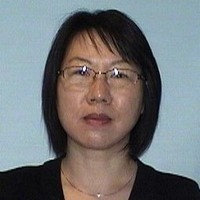
\includegraphics[width=.9\linewidth]{./pic/Sherry Wang.jpg}

\begin{itemize}
\item 97年之前我不清楚,但97年至2000零几年的夏天,王孔启都在他曾经的家乡湖北省襄阳市宜城市朱市镇镇上王孔庚的家过夏天。关于王夏华如果来美在美国如何才能够生存下来,他们两家人一族人应该是深思熟虑,就其可能性讨论过无数次了。
\begin{itemize}
\item 2005年秋冬我申请美国的学校,数年不曾谋面的王夏华父母赴美之前却还能在北京饭店里请我吃饭,并将我美国五所学校的申请材料随其旅行箱亲自带至美国加州再分寄出去。
\item 2005年我所申请的美国五所学校,都是Cindy Wang通过电子邮件推荐的,包括WSU和UI
\item 2006年秋我赴美读书,感恩节打电话至加州王夏华母亲处,其母电话里反复重申:他们早就已经告诉过王孔启我在旁边学校读书,怎么他还没有来找你?
\item 2008年夏天KC Wang王孔启带我至加州王秋勤Cindy Wang处大城市打工。说的是要带我去大城市打工,实则王孔启是传达要求王夏华好好利用我以使其在美国能够轻松生存下来之意。王孔启当着一众亲人的面,当着五夏华及其父母的面,拍着胸脯说他保证他能够发动他所能够发动的势力,以使他家五夏华能够在美国轻松地生存下来
\item 2008年夏天,王夏华父母当着KC Wang王孔启的面,告诉我,他们(王夏华的父亲和母校)绝对不会允许我放弃读博而转读硕士。经济担保我读硕士是王孔启KC Wang在祸害别人的人生。王孔启没有任何可反驳、反对的。
\item 2015年我回加州时,王秋勤还为王孔启说话,说其就是那么个拎不清。但她的说辞此地无银三百两。说到底,王孔启KC Wang就是故意作贱、祸害了别人的人生。

\item 未完待续
\end{itemize}
\end{itemize}

\section{关键人物:王夏华}
\label{sec-8}
\begin{itemize}
\item 97年之前我不清楚,但97年至2000零几年的夏天,王孔启KC Wang每年夏天都在他曾经的家乡湖北省襄阳市宜城市朱市镇镇上王夏华的父母王孔庚的家过夏天。关于相对于王秋勤来说要笨很多的王夏华如果来美在美国如何才能够生存下去,他们两家人一族人应该是深思熟虑,就其可能性讨论过无数次了。
\begin{itemize}
\item 2005年秋冬我申请美国的学校,数年不曾谋面的王夏华父母赴美之前却还能在北京饭店里请我吃饭,并将我美国五所学校的申请材料随其旅行箱亲自带至美国加州再分寄出去。
\item 2005年我所申请的美国五所学校,都是Cindy Wang通过电子邮件推荐的,包括WSU和UI
\item 2006年秋我赴美读书,感恩节打电话至加州王夏华母亲处,其母电话里反复重申:他们早就已经告诉过王孔启我在旁边学校读书,怎么他还没有来找你?
\item 2008年夏天KC Wang王孔启带我至加州王秋勤Cindy Wang处大城市打工。说的是要带我去大城市打工,实则王孔启是传达要求王夏华好好利用我以使其在美国能够轻松生存下来之意。王孔启当着一众亲人的面,当着五夏华及其父母的面,拍着胸脯说他保证他能够发动他所能够发动的势力,以使他家王夏华能够在美国轻松地生存下来。
\item 2008年夏天,王夏华父母当着KC Wang王孔启的面,告诉我,他们(王夏华的父亲和母校)绝对不会允许我放弃读博而转读硕士。经济担保我读硕士是王孔启KC Wang在祸害别人的人生。王孔启没有任何可反驳、反对的。
\item 2015年我回加州时,王秋勤还为王孔启说话,说其就是那么个拎不清。但她的说辞此地无银三百两。说到底,王孔启KC Wang就是故意作贱和祸害了别人的人生。
\item 王夏华父母为了他们的立场,在国内亲人场已经开始把王孔启说成是神经病。
\end{itemize}
\end{itemize}
\subsection{未达成她的愿望前,反复利用别人}
\label{sec-8-1}
\begin{itemize}
\item 2006年我来美读收后的第二年,2007年王夏华便从加拿大来到了美国,并在王秋勤的帮助下顺利地在Cisco得到了第一份工作,这份工作干了半年多的时间
\item 此后2008、2010年和2013、2015都反复和我说她工作上的事,她好感恩她工作上某个待她好的上级或同事,说她多想把她笨笨弄美国来,表现出一副多么感恩的样子。
\item 2015年王夏华将何/贺笨笨的简历递给当时正在苹果工作、也是2013年夏天王夏华和我在三星工作的组长并最终被苹果公司录用的事,王夏华当然坚定地认为是她王夏华的能耐和本事,得到的多么理直气壮,就像她被三星公司加持出差西雅图、被三星包养给办绿卡一样,和她招买保马车一样,理直气壮,全是她王夏华的能耐,呵呵。
\item 可是,当我问及她是否感激帮助她、使她极弱的背景能够在WSU读硕、以及帮她顺利拿到各种勤工俭学助学金的王孔启KC Wang时,王夏华说,“帮助别人的时候就别只想着求回报”,“再说,我读书的时候用的都是自己多年工作攒的钱和王秋勤的钱,他王孔启并不曾帮上我什么忙,我不需要感激他什么。”作为得到帮助的受益者,王夏华那段话说得还真是脸不红心不跳。
\item 2017年,当她2015年已被三星公司终身包养给办绿卡,她的儿子何/贺笨笨2015年也被空降至苹果,我与她再交往接触时,她王夏华的目的再次明确出来:故意口是心非地对她当时在加州的老公说,“你要么在这边找个工作,要么就在那边找个人过”。呵呵,利用人利用得、得到得都要成神仙了,美国政府是为她王夏华一家服务的!继把她儿子何笨笨空降到苹果之后,美国政府还该将她五六十岁的老公也空降至加州来!
\end{itemize}
\subsection{达成她的愿望后,过河折桥}
\label{sec-8-2}
\begin{itemize}
\item 2008年王孔启和我、王夏华及其父母都在王秋勤家时,王孔启所在的一周时间,王夏华故意逃避宿舍,每天晚上故意11点多才回家,待王孔启一走,她便恢复了八点钟左右就回到家
\end{itemize}
燕:
\section{关键人物:王夏华}
\label{sec-9}
\begin{itemize}
\item 97年之前我不清楚,但97年至2000零几年的夏天,王孔启KC Wang每年夏天都在他曾经的家乡湖北省襄阳市宜城市朱市镇镇上王夏华的父母王孔庚的家过夏天。关于相对于王秋勤来说要笨很多的王夏华如果来美在美国如何才能够生存下去,他们两家人一族人应该是深思熟虑,就其可能性讨论过无数次了。
\begin{itemize}
\item 2005年秋冬我申请美国的学校,数年不曾谋面的王夏华父母赴美之前却还能在北京饭店里请我吃饭,并将我美国五所学校的申请材料随其旅行箱亲自带至美国加州再分寄出去。
\item 2005年我所申请的美国五所学校,都是Cindy Wang通过电子邮件推荐的,包括WSU和UI
\item 2006年秋我赴美读书,感恩节打电话至加州王夏华母亲处,其母电话里反复重申:他们早就已经告诉过王孔启我在旁边学校读书,怎么他还没有来找你?
\item 2008年夏天KC Wang王孔启带我至加州王秋勤Cindy Wang处大城市打工。说的是要带我去大城市打工,实则王孔启是传达要求王夏华好好利用我以使其在美国能够轻松生存下来之意。王孔启当着一众亲人的面,当着五夏华及其父母的面,拍着胸脯说他保证他能够发动他所能够发动的势力,以使他家王夏华能够在美国轻松地生存下来。
\item 2008年夏天,王夏华父母当着KC Wang王孔启的面,告诉我,他们(王夏华的父亲和母校)绝对不会允许我放弃读博而转读硕士。经济担保我读硕士是王孔启KC Wang在祸害别人的人生。王孔启没有任何可反驳、反对的。
\item 2015年我回加州时,王秋勤还为王孔启说话,说其就是那么个拎不清。但她的说辞此地无银三百两。说到底,王孔启KC Wang就是故意作贱和祸害了别人的人生。
\item 王夏华父母为了他们的立场,在国内亲人场已经开始把王孔启说成是神经病。
\end{itemize}
\end{itemize}
\subsection{未达成她的愿望前,反复利用别人}
\label{sec-9-1}
\begin{itemize}
\item 2006年我来美读收后的第二年,2007年王夏华便从加拿大来到了美国,并在王秋勤的帮助下顺利地在Cisco得到了第一份工作,这份工作干了半年多的时间
\item 此后2008、2010年和2013、2015都反复和我说她工作上的事,她好感恩她工作上某个待她好的上级或同事,说她多想把她笨笨弄美国来,表现出一副多么感恩的样子。
\item 2015年王夏华将何/贺笨笨的简历递给当时正在苹果工作、也是2013年夏天王夏华和我在三星工作的组长并最终被苹果公司录用的事,王夏华当然坚定地认为是她王夏华的能耐和本事,得到的多么理直气壮,就像她被三星公司加持出差西雅图、被三星包养给办绿卡一样,和她招买保马车一样,理直气壮,全是她王夏华的能耐,呵呵。
\item 可是,当我问及她是否感激帮助她、使她极弱的背景能够在WSU读硕、以及帮她顺利拿到各种勤工俭学助学金的王孔启KC Wang时,王夏华说,“帮助别人的时候就别只想着求回报”,“再说,我读书的时候用的都是自己多年工作攒的钱和王秋勤的钱,他王孔启并不曾帮上我什么忙,我不需要感激他什么。”作为得到帮助的受益者,王夏华那段话说得还真是脸不红心不跳。
\item 2017年,当她2015年已被三星公司终身包养给办绿卡,她的儿子何/贺笨笨2015年也被空降至苹果,我与她再交往接触时,她王夏华的目的再次明确出来:故意口是心非地对她当时在加州的老公说,“你要么在这边找个工作,要么就在那边找个人过”。呵呵,利用人利用得、得到得都要成神仙了,美国政府是为她王夏华一家服务的!继把她儿子何笨笨空降到苹果之后,美国政府还该将她五六十岁的老公也空降至加州来!
\end{itemize}
\subsection{达成她的愿望后,过河折桥}
\label{sec-9-2}
\begin{itemize}
\item 2008年王孔启和我、王夏华及其父母都在王秋勤家时,王孔启所在的一周时间,王夏华故意逃避宿舍,每天晚上故意11点多才回家,待王孔启一走,她便恢复了八点钟左右就回到家
\item 此后2008、2010年和2013、2015都反复和我说她工作上的事,她好感恩她工作上某个待她好的上级或同事,说她多想把她笨笨弄美国来,表现出一副多么感恩的样子。2015年王夏华将何/贺笨笨的简历递给当时正在苹果工作、也是2013年夏天王夏华和我在三星工作的组长并最终被苹果公司录用的事,王夏华当然坚定地认为是她王夏华的能耐和本事,得到的多么理直气壮,就像她被三星公司加持出差西雅图、被三星包养给办绿卡一样,和她招买保马车一样,理直气壮,全是她王夏华的能耐,呵呵。可是,当我问及她是否感激帮助她、使她极弱的背景能够在WSU读硕、以及帮她顺利拿到各种勤工俭学助学金的王孔启KC Wang时,王夏华说,“帮助别人的时候就别只想着求回报”,“再说,我读书的时候用的都是自己多年工作攒的钱和王秋勤的钱,他王孔启并不曾帮上我什么忙,我不需要感激他什么。”作为得到帮助的受益者,王夏华那段话说得还真是脸不红心不跳。
\item 2017年,王夏华一边利用我希望能将她老公也搬到美国来,一边开始甩人。别人的目的基本都达到了,还要你这种被利用的人作什么呢,拆她的桩吗
\end{itemize}

燕:
\begin{itemize}
\item 她贺笨笨也并不是学习成绩有多好能去到苹果公司,他与他的同学一起面试时,他的同学可以过,他却过不了。最终,是2013年我假期实习时我和王夏华一个组里的组长当时在苹果工作,帮refer才与其说是看在王夏华的面子上,不如说是看在KC Wang政治投机,作贱了别人的人生来执行所谓的爱国的面子上,录取了贺笨笨到苹果公司工作。
\item 而在别人真真需要帮助的时候,她王夏华逃得比谁都快。2015年我在回州某学校读书经济不足,我和两个同学总共只能凑够八千块,想请她帮忙经济担保,她五夏华逃跑得比世人都快。想要得到她的帮助,门都没有。最终我只能请当时同一个房东的一个好心房客帮助我。而作为亲人的她王夏华,她哪怕有一点儿人情,又何至于逃之矢矢?
\item 2017年,贺笨笨的工作已经得到解决。我再与王夏华交往,她的目的转向她家老公,说得出做得出,寄希望美国政府继解决她家她自己的工作被三星公司包养、办绿卡、养老送终;继她儿子贺笨笨被苹果公司从加拿大直接空降至苹果公司工作之后,寄希望美国政府继解决她家她老公的工作,寄希望能把她五六十岁的老公也能像她儿子所得到的那样再被某个公司从加拿大空降至加州,她王夏华还真是神啊
\item 2017年,贺笨笨的工作已经得到解决。王夏华一边寄希望能把她老公也弄来,一边开始设甩人。2017年多少次她、并支使她家贺笨笨故意冷落敷衍我,赶人甩人,只因为她家已经得到了那么多的好处,她大部分的心愿已满足,我对于她来说已经不再有多的利用价值,只添后乱。所以一再设计甩人。
\end{itemize}

燕:
\subsection{自私自利,贪小便宜,只会利用别人,没有真情}
\label{sec-9-3}
\begin{itemize}
\item 她自私自利,贪图各种小便宜。2010年她要回中国前在301 Ranch walmart旁边的一家店买衣服,接近两百块的衣服钱想要欺负我要我付账,是店员作主逼着她自己付账,而不是像她希望的那样利用我要我帮她付;2013年夏天在costco买花也就\$15块左右,她却想要不付账偷偷拿跑,被抓个现形,乖乖回去付账。
\item 她的一丁点儿人情,不过是赤裸裸地利用。2015年她的绿卡问题得到解决,但她的儿子贺笨的工作还没有,她奸吝地带我去看一个门版号947的房间,后院里改造的简陋小平房,旁边有游泳池,吵得要死,非要别人住那。她就是奸吝,想要继续利用我好能为她家贺笨笨的解决工作而已。
\item 我的一生大部分时光都呆在校园,2013年我对形势还并不清楚。自2007年参加工作、2008年夏天她的小叔KC Wang特意点醒,她与自己的妹妹Cindy Wang共同有商有量,显然对形势比我清楚多了。当着我聊天时一再标榜她自己有多能干,而实际她王夏华当时在三星公司的状态不过是被公司养着,没有什么多的项目做,相当于给她时间自己学习充电而已。我被她利用最终使得公司开走了组里另一个人,把她留下,她买豪车,却反映的正是她骨子里的自卑:她笨,学习成绩不好,大学都要考两年,考得还不是大学本科,一个大专而已;只能靠她小叔残忍地祸害别人的人生、以政治投机的手段才使得她一家得以在美国生存下来。

\item 而王夏华的更邪恶之外就在于,把别人往别人小三情妇的角色上推。
\begin{itemize}
\item 我九几年在王夏华父母家看的第一部电影,便是其父母为我选择的《魂断蓝桥》,一个女孩因为战争沦为妓女的故事。
\item 魔蝎座的王夏华本人是银荡的,二十多岁上交往多年的男朋友出车祸眼睛瞎了,她便果断与之分手,并女追男追到了原本对她远在美国的妹妹王秋勤有意思的其妹妹的同学贺某。2009、2010年期间还与其公司的男同事牵牵连连藕断丝连;其通过某种直觉、又或者父辈的社会阅历(或他们两家人讨论王夏华在美国能够生存下来的手段讨论出来的我的出路?)、常年生活在加州意识到我能出名是三大中文网站故意炒作的结果,了解到贵圈很乱,便变着方的想要把我朝那条路上推,以断绝我一切可能回复的可能性,和大环境再把她牵连其中、再要求其回报王孔启的一切可能性。2013年8月我工作的最后一天便把组里的人带到了三大中文网站的大本营窝点;2015年带我去Montery还说是为了帮助我能当上别人的小三给我壮面子。呵呵,她居然还能够说得出这种话。这便是她王夏华作为一个远亲表姐为了她自己的自私自利便能轻轻松松做得出来的事。
\end{itemize}
\end{itemize}

而王夏华现在在三星、其儿子在苹果公司的存大便的的确确地成了过去妓院老么么般皮条客的存在。这样的人不被逼,三大媒体还有脸来逼我,只能说明:三大逼良为娼野心毕现!它同样的那份伎俩使用一千次能得手,并不能证明,它同样的伎俩在我这里能够得手。而我要做的,正是让全世界都认识到三大中文媒体逼良为娼的本质

?她设计让我发动自己的亲姐妹去看望她在国内身体稍有不适的父母后,却转眼对别人的病不闻不问,没有关心,没有探望。
\begin{itemize}
\item 她的奸诈就在于,为了得到她自己和她家何笨笨工作上的帮助,她最初2010年时故意给我介绍男朋友,说王孔启KC Wang家老二是个不适合也不会结婚的;2015年她被三星公司故意加持出了次差并给办了绿卡之后、在她儿子被空降苹果之前,她还又故意悭吝地带别人去看去租个什么门版号是947的房间;至2017年我与现任老公结婚后,她嘴里说着我怎么选都可以,实则一次又一次地利用开车有噪音背景的机会,一次又一次地劝我,在美国怎么都能生存下去,别人修理门窗的都能生存下去,你读了这么多的书还怕生存不下去吗?其狼子野心的目的,不过是避免一切可能的将来需要回报王孔启KC Wang的可能性。而王夏华这一切飞黄腾达的背后,都是建立在王孔启KC Wang对别人人生的故意践踏。
\end{itemize}
% Emacs 27.1 (Org mode 8.2.7c)
\end{document}